\documentclass[11pt]{article}
\usepackage{listings,amsmath,amssymb,bbm}
\usepackage{amsthm}
\usepackage{graphicx}
\usepackage{color}
\usepackage{multirow}
\usepackage{natbib}
\oddsidemargin0cm
\topmargin-1.4cm
\textheight23.5cm
\textwidth16cm
\parindent0cm
\renewcommand{\baselinestretch}{1.1}
\numberwithin{equation}{section}
\lstset{language=R,basicstyle=\ttfamily\footnotesize,breaklines=true}
\usepackage{booktabs}
\def\R{{\mathbb R}}  %%
\def\N{{\mathbb N}}  %%
\def\E{{\mathbb E}}  %%
\def\Z{{\mathbb Z}}  %%
\def\bc{\boldsymbol{c}}
\def\bd{\boldsymbol{d}}
\def\bx{\boldsymbol{x}}
\def\bm{\boldsymbol{m}}
\def\by{\boldsymbol{y}}
\def\bZ{\boldsymbol{Z}}
\def\bz{\boldsymbol{z}}

\newcounter{saveenumi}
\newcommand{\seti}{\setcounter{saveenumi}{\value{enumi}}}
\newcommand{\conti}{\setcounter{enumi}{\value{saveenumi}}}

\newcommand{\blue}[1]{\textcolor{blue}{#1}}
\newcommand{\red}[1]{\textcolor{red}{#1}}
\usepackage{url}%For ref url
%\bibliographystyle{plain}
%opening
\title{Insurance loss modeling with gradient tree-boosted mixture models.}
\author{Guangyuan Gao \and Jiahong Li}


\begin{document}

\maketitle

\begin{abstract}
Sometimes insurance loss data cannot be well modeled by a single distribution. Mixture of models are often applied in insurance loss modeling. 
The Expectation-Maximization (EM) algorithm is usually applied for parameter estimation in mixture of models. 
Feature engineering and variable selection are challenging for mixture of models due to several component models involving. 
Overfitting is also a concern when predicting future loss. 
To address those issues, we propose an Expectation-Boosting (EB) algorithm, 
which replaces the maximization step in the EM algorithm by a gradient boosting with decision trees. 
The boosting algorithm estimates the regression functions in component models non-paramerically and overfitting-sensitively. 
The EB algorithm performs automated feature engineering, model fitting and variable selection simultaneously, 
fully exploring the predictive power of covariate space.
Simulations show that the proposed method performs very well.
An empirical analysis of the claims amounts data is illustrated for the proposed methodology. 

\end{abstract}

{\bf Keywords:} Mixture models; EM algorithm; Gradient boosting.


\section{Introduction}

Insurance loss data sometimes cannot be well modelled by a single distribution.
For claim count data, it may have an excess of zero claims, so a Poisson distribution may not be the best option.
For claim amount data, its probability density function may be multimodal or heavy tailed, so a gamma distribution is not enough to describe the entire data.
One solution to such issues is to apply mixture of distributions.
When the individual risk factors are available, the mixture of distributions can be extended to mixture of regressions to address the risk heterogeneity in the portfolio.
Mixture model is proposed by \citet{goldfeld1973markov}.
We refer to \citet{lindsay1995mixture} and \citet{peel2000finite} for detailed review of mixture models.
In machine learning applications, mixture models are also called as mixture of experts models \citep{jacobs1991adaptive,jiang1999hierarchical}.

Mixture models have been used for insurance loss modeling frequently.
\citet{zhang2020type, zhang2022new} developed a multivariate zero-inflated hurdle model to describe multivariate count data with extra zeros.
\citet{delong2021gamma} propose a mixture of neural networks with gamma loss to model insurance claim amounts.
\citet{verbelen2015fitting} and \citet{lee2010modeling} used mixture of Erlangs to model insurance claim amounts including censored and truncated data.
\citet{lee2012modeling} developed the multivariate version of mixture Erlangs.
\citet{fung2019class}, \citet{fung2019class2} and \citet{tseung2021lrmoe} developed a so called logit-weighted reduced mixture of experts models for multivariate claim frequencies or severities distributions.
To the best of our knowledge, the existing studies always impose a linear constraint on the regression function, i.e., under a generalized linear model framework.
In this paper, we will relax this constraint by estimating regression function nonparametrically.

Parameter estimation in mixture models is challenging since component parameters are related to each other. 
The Expectation-Maximization (EM) algorithm proposed by \citet{dempster1977maximum} is an iterative method to estimate component parameters and (hidden) component indicator variable. 
Variable selection and feature engineering in mixture models  is also challenging since the relationship between covariates and response vary from one component to another.  
\citet{khalili2007variable} introduced a penalized likelihood approach for variable selection.
\citet{huang2013nonparametric} and \citet{huang2012mixture} proposed nonparametric mixture of regression to relax the linearity assumption on the regression function.
Selecting the number of components is another challenging problem.
\citet{naik2007extending} derived a new information criterion for selection of component numbers and variables.
\citet{kasahara2015testing} proposed a likelihood-based test to contrast mixture models with different numbers of components. 

In this paper, we propose an Expectation-Boosting (EB) algorithm, which replaces the maximization step by an overfitting-sensitive boosting step. 
There are several advantages of EB algorithm over the EM algorithm. 
First, boosting algorithm is a flexible non-parametric regression facilitating both non-linear effects and interaction. 
Second, boosting algorithm is overfitting-sensitive. With decision tree as weak learner, we can perform variable selection simultaneously. 
Boosting algorithm is an iteration method to estimate weak learners step-wisely.
It has a close relationship with the additive model.
Commonly used boosting algorithms are listed below
	\begin{enumerate}
		
		\item Binary classification: {AdaBoost}, LogitBoost (real, discrete, gentle AdaBoost), AdaBoost.M1
		
		\item Multinomial classification: Stagewise Additive Modeling using a Multi-class Exponential loss (SAMME), SAMME.R (multi-class real AdaBoost),
		\item {Gradient based}: {gradient boosting machine/model (GBM)}, Newton boosting, gradient boosting decision tree (GBDT), {eXtreme Gradient Boosting (XGBoost)}, {light gradient boosting machine (LightGBM)}
	\end{enumerate}
The last type is based on {gradient of loss function} \citep{friedman2001greedy}, and our EB algorithm uses this version of boosting.

The paper is structured as follows. Section \ref{sec:review} reviews mixture of models and the EM algorithm. Section \ref{sec:EB} proposes the EB algorithm. Section \ref{sec:application} studies two simulated data and a real data to illustrate the proposed methodology. Section \ref{sec:conclusions} concludes the paper with several important findings.  


\section{Review: mixture of models and the EM algorithm}\label{sec:review}


\subsection{Mixture of models}\label{review:mix1}
In this paper, we focus on the exponential distribution family with expectation parameter $\mu$ and dispersion parameter $\phi$. The exponential distribution family is normally sufficient to fit to most insurance loss data.
	Suppose a random variable $y$ follows the $k$-th {\it component distribution} from
	$$\{f_1(y;\mu_1,\phi_1),\ldots,f_K(y;\mu_K,\phi_K)\}$$
	with \textit{mixing probability} $p_k, k=1,\ldots,K$,
	then the probability density function for $y$ is
	$$f(y)=\sum_{k=1}^Kp_kf_k(y;\mu_k,\phi_k).$$

	If {\it individual features $\bx_i$} are available and they have systematic effects on the distribution of $y_i$, then we establish a mixture of regressions:
	$$f(y|\bx)=\sum_{k=1}^Kp_k(\bx)f_k(y;\mu_k(\bx),\phi_k(\bx)).$$
	
	Above is the most general form of mixing. In applications, we always put some constraints on the \textit{mixing structure}:
	
	\begin{itemize}
		\item Mixing probabilities are not related to $\bx$
		$$f(y)=\sum_{k=1}^Kp_kf_k(y;\mu_k(\bx),\phi_k(\bx)).$$
		\item Both mixing probabilities and dispersions are not related to $\bx$
		$$f(y)=\sum_{k=1}^Kp_kf_k(y;\mu_k(\bx),\phi_k),$$

		\item If component distributions are from the same distribution family, we might assume different component distributions have the same dispersion $\phi$
		$$f(y)=\sum_{k=1}^Kp_kf_k(y;\mu_k(\bx),\phi).$$
		\item Covariates $\bx$ are only related to the mixing probabilities:
		$$f(y)=\sum_{k=1}^Kp_k(\bx)f_k(y;\mu_k,\phi_k).$$
	\end{itemize}
	
	We need to determine the mixture structure according to the data and our aim. Imposing suitable constraints on mixture, we can {accelerate model fitting} without compromising predictive performance.

\subsection{EM algorithm}

	Suppose that we know which component distribution $f_k$ each sample $y$ is from. That is we know the \textit{full information} $(Y,\bZ,\bx)$ where
	$$\bZ=(Z_1,\ldots,Z_K)^\top=(\mathbbm{1}_1(k),\ldots,\mathbbm{1}_K(k))^\top$$
	is the one-hot encoding of \textit{component indicator variable}.
	The joint distribution function for full information (one sample) is given by
	$$f(y,\bz|
	\bx) = \prod_{k=1}^K\left[p_k(\bx)f_k(y;\mu_k(\bx),\phi_k(\bx))\right]^{z_k}$$
	The {log-likelihood function} is given by
	\begin{equation}\label{full-L}
		l(p,\mu,\phi|y,\bz,\bx)=\sum_{k=1}^K z_k\left[\log p_k(\bx) + \log f_k(y;\mu_k(\bx),\phi_k(\bx))\right]
	\end{equation}
	Given a data set $(y_i,\bz_i,\bx_i)_{i=1:n}$, the regression coefficients $\theta_p, \theta_\mu, \theta_\phi$ in $p,\mu,\phi$ can be estimated by the following $K+1$ {independent optimizations}
	\begin{equation}\label{p-reg}
		\hat{\theta}_p=\underset{\theta_p}{\arg\max}\sum_{i=1}^n\sum_{k=1}^Kz_{i,k}\log p_k(\bx_i;\theta_p)
	\end{equation}
	\begin{equation}\label{comp-reg}
		\left(\hat{\theta}_\mu^{(k)},\hat{\theta}_\phi^{(k)}\right)=\underset{\theta^{(k)}_\mu,\theta^{(k)}_\phi}{\arg\max}\sum_{i=1}^n\sum_{k=1}^Kz_{i,k}\log f_k\left(y_i;\mu_k\left(\bx_i;\theta_\mu^{(k)}\right),\phi_k\left(\bx_i;\theta_\phi^{(k)}\right)\right), ~\text{for} ~ k=1,\ldots,K.
	\end{equation}
	Those optimizations are corresponding to  {\it a multinomial logistic classification} and {\it $K$ regressions}.
Note that the multinomial logistic classification \eqref{p-reg} are fitted to all samples, while $K$ regressions \eqref{comp-reg} are fitted to {partial} samples with $\{i:z_{i,k}=1\}$.
In practice we do not have full information  $(Y,\bZ,\bx)$ but only the incomplete information $(Y,\bx)$. The following EM algorithm is inspired by the above discussion.
\paragraph{Expectation step.}
	With iterated $\hat{p},\hat{\mu},\hat{\phi}$, calculate the \textit{conditional expectation} of $\bz$:
	$$\hat{z}_{i,k}=\hat{z}_k(\bx_i)=\frac{\hat{p}_{i,k}f_k(y_i;\hat{\mu}_{i,k},\hat{\phi}_{i,k})}{\sum_{l=1}^K\hat{p}_{i,l}f_l(y_i;\hat{\mu}_{i,l},\hat{\phi}_{i,l})},$$
	where
	$\hat{p}_{i,k}=\hat{p}_k(\bx_i)= p_k(\bx_i;\hat{\theta}_p),\hat{\mu}_{i,k}=\hat{\mu}_k(\bx_i)=\mu_k\left(\bx_i;\hat{\theta}_\mu^{(k)}\right),\hat{\phi}_{i,k}=\hat{\phi}_k(\bx_i)=\phi_k\left(\bx_i;\hat{\theta}_\phi^{(k)}\right)$.

\paragraph{Maximization step.}
	Based on the following likelihood function for full information, calculate the MLE of regression coefficients  $\theta_p, \theta_\mu, \theta_\phi$.
	\begin{equation}
		\begin{aligned}
			&l(p,\mu,\phi|y,\hat{z},\bx)\\
			=&\sum_{i=1}^n\sum_{k=1}^K \hat{z}_{i,k}\left[\log p_k(\bx_i;\theta_p) + \log f_k\left(y_i;\mu_k\left(\bx_i;\theta_\mu^{(k)}\right),\phi_k\left(\bx_i;\theta_\phi^{(k)}\right)\right)\right]\\
			=&\sum_{i=1}^n\sum_{k=1}^K \hat{z}_{i,k}\log p_k(\bx_i;\theta_p) + \sum_{i=1}^n\sum_{k=1}^K \hat{z}_{i,k}\log f_k\left(y_i;\mu_k\left(\bx_i;\theta_\mu^{(k)}\right),\phi_k\left(\bx_i;\theta_\phi^{(k)}\right)\right)
		\end{aligned}
	\end{equation}
	This step is similar to \eqref{p-reg} and \eqref{comp-reg}. However, now we have $\hat{z}_{i,k}\in(0,1)$, 
	so we need to consider a multinomial logistic classification with {fractional} response and $K$ {weighted}-regressions fitted to {all} samples.

\section{Expectation-Boosting algorithm}\label{sec:EB}
We replace the maximization step in the EM algorithm by a boosting step. The boosting step increases the likelihood in each iteration, but overfitting-sensitively.
The boosting step follows a generic functional gradient descent algorithm.
We first review generic functional gradient descent algorithm, then describe our proposed EB algorithm.

\subsection{Generic functional gradient descent algorithm}

	Suppose a {non-parametric regression function} as $F:\R^P\rightarrow\R$. Our purpose is to  estimate $F$ to minimize the expected loss $$\hat{F}=\underset{F}{\arg\min}\E\left[C(Y,F(\bx))\right],$$
	where $C:\R\times\R\rightarrow\R_+$ is the \textit{loss function}.
	We always replace the expected loss by sample average loss:
	$$\hat{F}=\underset{F}{\arg\min} \frac{1}{n}\sum_{i=1}^nC(y_i,F(\bx_i))$$
	We choose the \textit{negative log-likelihood} function as the loss function. Hence, minimizing the loss function is equivalent to maximizing the likelihood function.
The link function is used to link the regression function $F$ with the parameter interested such as mean, probability odds, etc. 
	Commonly used {link function} and loss functions in different boosting algorithms are listed below:
	\begin{itemize}
		\item AdaBoost: $$C(y,F)=\exp(yF),  ~~ y\in\{-1,1\}$$
		$$F(\bx)=\frac{1}{2}\log\left(\frac{\Pr[Y=1|\bx]}{\Pr[Y=-1|\bx]}\right)$$
		\item LogitBoost: $$C(y,F)=\log_2(1+\exp(-2yF)), ~~ y\in\{-1,1\}$$
		$$F(\bx)=\frac{1}{2}\log\left(\frac{\Pr[Y=1|\bx]}{\Pr[Y=-1|\bx]}\right)$$
		\item $L_2$Boost: 
		\begin{equation}\label{l2}
			C(y,F)=(y-F)^2/2, ~~ y\in \R
		\end{equation}
		$$F(\bx)=\E(Y|\bx)$$
	\end{itemize}

We follow \citet{buehlmann:2003} to review the generic functional gradient decent algorithm:

	\begin{enumerate}
		\item Initialization: $\hat{F}^{[0]}(\bx;\hat{\theta}^{[0]}),$ where $\hat{\theta}^{[0]}$ are determined by $(y_i,\bx_i)_{i=1:n}$.
		Let $m=0.$
		\item Projection of gradient to weak learner:
		Calculate \textit{negative gradient} $$u_i=\left.-\frac{\partial C(y_i,F)}{\partial F}\middle|_{F=\hat{F}^{[m]}(\bx_i)}\right., i=1,\ldots,n.$$
		Data $(u_i,\bx_i)_{i=1:n}$ is used to calibrate a weak learner $\hat{f}^{[m+1]}(\bx;\hat{\theta}^{[m+1]})$ with \textit{loss function $L_2$} \eqref{l2}.
	
		\item One-dimensional optimization:
		Solve an one-dimensional optimization  to find \textit{expansion coefficient} $\hat{\omega}^{[m+1]}$:
		$$\hat{\omega}^{[m+1]}=\underset{\omega}{\arg\min}\sum_{i=1}^n C(y_i, \hat{F}^{[m]}(\bx_i)+\omega\hat{f}^{[m+1]}(\bx_i))$$
		Update $$\hat{F}^{[m+1]}=\hat{F}^{[m]}+s\hat{\omega}^{[m+1]}\hat{f}^{[m+1]},$$
		where $s$ is \textit{shrinkage factor} (learning rate).
		\item Iteration: Let $m$ increase by 1, and repeat steps 2-3.
			\end{enumerate}
In the algorithm, weak learners are fitted to negative gradient $U$ rather than $Y$.
		 Loss function in weak learners is always $L_2$, independently with model loss function $C$. 
		 If weak learners are trees, the algorithm is called \textit{gradient boosting decision tree (GBDT)}, and {calibration and variable selection} are performed simultaneously.
		\citet{buhlmann2007boosting} argue that step 3 of one-dimensional optimization seems unnecessary given learning rate $s$ is sufficiently small according to some empirical experiments.




\subsection{Expectation-Boosting algorithm}

We denote the regression functions for the interested parameters $p,\mu,\phi$ by {$F,G,H$}. In the EB algorithm, we need to specify link functions and cost/loss functions, which determines negative gradient function.
For mixing probabilities $p$, we choose multiple logistic link function for mixing probabilities.	
	\begin{equation}\label{logistic}
		p_k(F(\bx))=\Pr(Z_k=1|\bx)=\frac{\exp{F_k(\bx)}}{\sum_{l=1}^{K}\exp{F_l(\bx)}},
	\end{equation}
	or equivalently
	\begin{equation}\label{inv-logistic}
		F_k(\bx)=\log p_k(\bx)-\frac{1}{K}\sum_{l=1}^K\log p_l(\bx),~~k=1,\ldots,K.
	\end{equation}
We use the negative log-likelihood function as the cost function
\begin{equation}
	\begin{aligned}
		{C_{Z}(\bZ, F(\bx))}=& - \sum_{k=1}^K Z_k \log p_k(\bx).
	\end{aligned}
\end{equation}
The negative gradient of the cost function w.r.t. $F_k$ is given by
\begin{equation}
	{U_k(\bZ,F(\bx))}=-\frac{\partial C_{Z}(\bZ,F(\bx))}{\partial F_k(\bx)}=
	Z_k-p_k(\bx), ~~k=1,\ldots,K
\end{equation}

For component parameters $\mu$ and $\phi$, the link function and cost function (distribution) depend on the loss data.
Commonly used link functions in component models are indicated as follows
	\begin{itemize}
		\item Component Gaussian model:
		$$\mu_k(G_k(\bx))=G_k(\bx)$$
		$$\phi_k(H_k(\bx))=\exp H_k(\bx)$$
		\item Component Poisson model:
		$$\mu_k(G_k(\bx))=\exp G_k(\bx)$$
		\item Component gamma model:
		$$\mu_k(G_k(\bx))=\exp G_k(\bx)$$
		$$\phi_k(H_k(\bx))=\exp H_k(\bx)$$
	\end{itemize}
Note that we slightly abuse function notations $p_k,\mu_k,\phi_k$ (i.e. the inverse link function); in Section \eqref{review:mix1} they define different functions.
The negative log-likelihood function of each component model is used as its cost function:
	\begin{equation}
		\begin{aligned}
			{C_k(Y,\bZ,G_k(\bx))}=& -Z_k\log f_k(Y;\mu_k(G_k(\bx)),\phi_k), ~ k=1:K.
		\end{aligned}
	\end{equation}
	The negative gradient of $C_k$ w.r.t. $G_k$ is given by 
	$${V_k(Y,\bZ,G_k(\bx))}=-\frac{\partial C_k(Y,\bZ,G_k(\bx))}{\partial G_k(\bx)}.$$
	Note that we have assumed that dispersion $\phi_k$ is fixed among samples (not related to $\bx$) to avoid lengthy notations. The extension to dispersion modelling is straightforward; please refer to the real data analysis in Section ??.

Upon the above defined notations, we are ready to introduce the proposed EB algorithm.
We first summarize the proposed EB algorithm as follows, then we detail each step.
\begin{enumerate}
	\item[1] Initialization of EB algorithm $\hat{p}^{[0]},\hat{\mu}^{[0]},\hat{\phi}^{[0]}$. Set $t=0$.
	
	\item[2] Calculating conditional expectation of latent variable $\hat{z}^{[t]}$ given $\hat{p}^{[t]},\hat{\mu}^{[t]},\hat{\phi}^{[t]}$.
	
	\item[3.1]  Gradient boosting mixing probabilities $\hat{p}^{[t+1]}$  given latent variable $\hat{z}^{[t]}$.
	\item[3.2] Gradient boosting component model parameters $\hat{\mu}^{[t+1]}$ given latent variable $\hat{z}^{[t]}$.
	\item[4]  Calculate the MLE $\hat{\phi}^{[t+1]}$. Increase $t$ by 1. Repeat steps 2-3 until $t$ reaches to $T$.
	
\end{enumerate}
Note that we can perform steps 3.1 and 3.2 simultaneously by parallel computing which dramatically save running time.  Also note that  in the algorithm we have assumed that dispersion $\phi_k$ is fixed among samples (not related to $\bx$). The extension to dispersion modelling is straightforward by adding another gradient boosting step 3.3 for component model parameter $\phi$ and removing the MLE calculation in step 4.
	
In step 1 of initialization of EB algorithm, we neeed to initialize the following quantities.
	\begin{enumerate}
		\item[1.1] Initialize $\hat{p}_1^{[0]}, \ldots,\hat{p}_K^{[0]}$ and   $\hat{F}_1^{[0]}, \ldots, \hat{F}_{K}^{[0]}$:
		
		\begin{itemize}
			\item 	$\hat{p}_k^{[0]}=\frac{1}{K}$
			\item $\hat{F}_1^{[0]}, \ldots, \hat{F}_{K}^{[0]}$ are obtained by \eqref{inv-logistic}.
		\end{itemize}
		\item[1.2]
		Initialize $\hat{\mu}_1^{[0]},\ldots,\hat{\mu}_K^{[0]}$ and  $\hat{G}_1^{[0]},\ldots,\hat{G}_K^{[0]}$:
		
		\begin{itemize}
			\item $\hat{\mu}_k^{[0]}=\frac{\sum_{i=1}^nY_i}{n}$
			\item $\hat{G}_k^{[0]}=\mu_k^{-1}(\hat{\mu}_k^{[0]})$
		\end{itemize}
		\item[1.3] Initialize $\hat{\phi}_1^{[0]},\ldots, \hat{\phi}_K^{[0]}$ as the sample variance. (Assume that dispersion is independent with covariates.)
		\item[1.4] 	Set $t=0$.
	\end{enumerate}
	

In step 2 of conditional expectation of latent variable, we set  $\hat{z}_{i,k}^{[t]}$ as
	\begin{equation*}
		\hat{z}_{i,k}^{[t]}=\frac{\hat{p}_{k}^{[t]}(\bx_i) f_{k}\left(y_i ; \hat{\mu}_{k}^{[t]}(\bx_i), \phi_k^{[t]} \right)}{\sum_{l=1}^{K} \hat{p}_{l}^{[t]}(\bx_i) f_{l}\left(y_i ; \hat{\mu}_{l}^{[t]}(\bx_i), \phi_l^{[t]}\right)},~~ k=1:K.
	\end{equation*}


In step 3.1 of gradient boosting mixing probabilities, we implement a  multinomial logistic classification boosting with fractional response: 
	\begin{enumerate}
		\item[3.1.1] Initialization. Set $\hat{p}_1^{[t,0]}, \ldots, \hat{p}_K^{[t,0]}$ and $\hat{F}_1^{[t,0]}, \ldots, \hat{F}_{K}^{[t,0]}$ as
		\begin{equation}\label{ini-1}			
		\hat{p}_k^{[t,0]}=\frac{1}{K},
		~~\hat{F}_k(\bx)^{[t,0]}=\log \hat{p}_k^{[t,0]}-\frac{1}{K}\sum_{l=1}^K\log \hat{p}_l^{[t,0]}
	\end{equation}
		Set $m=0$.
		\item[3.1.2] Projection of gradient to learner.
		Compute the negative gradient sample $u_{1,k}^{[t,m]},\ldots,u_{n,k}^{[t,m]}$,  in which
		$$u_{i,k}^{[t,m]}=U_k(\hat{\bz}_{i}^{[t]},\hat{F}^{[t,m]}(\bx_i))=\hat{z}_{i,k}^{[t]}-\hat{p}_{i,k}^{[t,m]}.$$
		For each $k$, the data $(u_{i,k}^{[t,m]},\bx_i)_{i=1:n}$ is used to calibrate a $L$-terminal node regression trees $\hat{f}_k^{[t,m+1]}\left(\bx;R^{[t,m+1]}_{l=1:L},\bar{u}^{[t,m+1]}_{l=1:L}\right)$ with $L_2$ loss,
		where $R^{[t,m+1]}_{l=1:L}$ is the partition of covariate space and $\bar{u}^{[t,m+1]}_{l=1:L}$ contains the average gradient in each terminal node.
		
		
	
		\item[3.1.3]  The one-dimensional optimization for expansion coefficient leads to the following update \citep{friedman2001greedy}:
		
		$$\hat{F}_k^{[t,m+1]}(\bx_i)=\hat{F}_k^{[t,m]}(\bx_i)+s\sum_{l=1}^L\gamma^{[t,m+1]}_l\mathbbm{1}(\bx\in R^{[t,m+1]}_l),~ k=1,\ldots,K$$
		where
		$$\gamma^{[t,m+1]}_l=\frac{K-1}{K}\frac{\sum_{\bx_i\in R_l^{[t,m+1]}}u_{i,k}^{[t,m]}}{\sum_{\bx_i\in R_l^{[t,m+1]}}|u_{i,k}^{[t,m]}|(1-|u_{i,k}^{[t,m]}|)}$$
		We then derive the updated mixing probability $\hat{p}^{[t,m+1]}_{k=1:K}$  using \eqref{logistic}.
		
		
	
		\item[3.1.4] Increase $m$ by 1, and repeat steps 3.1.2-3.1.3  until $m$ reaches to the pre-determined $M_p$.
		Set $$\hat{F}_k^{[t+1]}=\hat{F}_k^{[t,M_p]},~~\hat{p}_k^{[t+1]}=\hat{p}_k^{[t,M_p]},$$
	\end{enumerate}
Note that  $K$ regression trees are fitted independently in step 3.1.2. We can accelerate this step by parallel computing.

In step 3.2 of gradient boosting component models, we implement $K$ weighted boosting:
	\begin{enumerate}
		\item[3.2.1] Initialization. Set $\hat{\mu}_1^{[t,0]},\ldots,\hat{\mu}_K^{[t,0]}$ and $\hat{G}_1^{[t,0]},\ldots,\hat{G}_K^{[t,0]}$:
			\begin{equation}\label{ini-2}
				\hat{\mu}_k^{[t,0]}=\frac{\sum_{i=1}^nY_i}{n}, \hat{G}_k^{[t,0]}=\mu_k^{-1}(\hat{\mu}_k^{[t,0]}).
			\end{equation}
		
		Set $m=0$.
		\item[3.2.2] Projection of gradient to learner.
		Compute the negative gradient samples $v_{1,k}^{[t,m]},\ldots,v_{n,k}^{[t,m]}$, in which
		$$v_{i,k}^{[t,m]}=V_k(y_i,\hat{\bz}^{[t]}_{i},\hat{G}^{[t,m]}(\bx_i)),$$
		For each $k$, the data $(v_{i,k}^{[t,m]},\bx_i)_{i=1:n}$ is used to calibrate a $L$-terminal node regression trees $\hat{g}_k^{[t,m+1]}\left(\bx;S^{[t,m+1]}_{l=1:L},\bar{v}^{[t,m+1]}_{l=1:L}\right)$ with $L_2$ loss, where $S^{[t,m+1]}_{l=1:L}$ is the partition of covariate space and $\bar{v}^{[t,m+1]}_{l=1:L}$ contains the average gradient in each terminal node.
		
	
	
		\item[3.2.3]  Conduct the following $K$ independent one-dimensional optimizations to find the best expansion coefficients.
		$$\hat{w}_{k}^{[t,m+1]}=\underset{w}{\arg\min}\sum_{i=1}^n C_{k}(y_i,\hat{\bz}_i^{[t]},\hat{G}_k^{[t,m]}(\bx_i)+w\hat{g}_k^{[t,m+1]}(\bx_i)).$$
		
		\item[3.2.4]  For each $k$, compute the updates
		$$\hat{G}_k^{[t,m+1]}(\bx_i)=\hat{G}_k^{[t,m]}(\bx_i)+s\hat{w}_{k}^{[t,m+1]}\hat{g}_{k}^{[t,m+1]}(\bx_i),$$
		$$\hat{\mu}_k^{[t,m+1]}(\bx_i)=\mu_k(\hat{G}_k^{[t,m+1]}(\bx_i)).$$
		\seti


		\item[3.2.5] Increase $m$ by 1, and repeat steps 3.2.2-3.2.4 until $m$ reaches to the pre-determined $M_\mu$. Set
		$$\hat{G}_k^{[t+1]}=\hat{G}_k^{[t,M_\mu]},~~\hat{\mu}_k^{[t+1]}=\hat{\mu}_k^{[t,M_\mu]}.$$
	\end{enumerate}
Note that $K$ independent boosting are implemented in step 3.2, we can accelerate this step by parallel computing.
	
In step 4, 
%for parameters not related to covariate $\bx$, 
compute the MLE $\hat{\phi}_k^{[t+1]}$ given all the other parameters $\hat{p}_k^{[t+1]}, \hat{\mu}_k^{[t+1]}$, then increase $t$ by 1 and repeat steps 2-3 until $t$
		reaches to the pre-determined $T$.
		
In the EB algorithm, we have the following tuning parameters and the corresponding tuning strategies are listed below:
	\begin{itemize}
		\item Number of EB iterations {$T$} (iterations in outer loop). This can be determined by screening the trace plot of loss.
		\item Number of iterations in boosting {$M_p,M_\mu$} (iterations in inner loops). We can specify a sufficiently large $M_p,M_\mu$ and use  early stop according to validation loss.
		\item Learning rate {$s$}. Smaller learning rate tends to lead to a better fitting and predictive performance but requiring more inner iterations.
		\item Tuning parameters in base learner tree: complexity parameter, maximum depth, number of terminal nodes. Those parameters can be tuned as in typical decision trees.
	\end{itemize}

		
{\bf Remarks.}
	In initialization of boosting steps 3.1.1 and 3.2.1, we initialize parameters {independently} with the previously boosting estimates $\hat{p}_k^{[t-1]}, \hat{\mu}_k^{[t-1]}$; see equations \eqref{ini-1} and \eqref{ini-2}. We call this as independent boosting.
	In contrast, we might initialize parameters as the previously boosted estimates $$\hat{p}_k^{[t,0]}=\hat{p}_k^{[t-1]}, \hat{\mu}_k^{[t,0]}=\hat{\mu}_k^{[t-1]}.$$
		This would lead a {smaller} required inner boosting iterations $M$ (or a {earlier} stop on validation loss). 
	We call this as forward boosting. 
	However, with forward boosting, it is difficult to predict for new data due to the {iterative initialization}. One solution is to apply an additional boosting with default initialization \eqref{ini-1} and \eqref{ini-2} given the {last expected hidden variables $\hat{\bz}_i^{[T]}$}. In the following applications, we only implement the independent boosting.
			
\section{Applications}\label{sec:application}

We conduct two simulated data analysis and a real data analysis. 
The first simulated data follows a mixture of Gaussian models. 
We use this example to illustrate the advantages of the EB algorithm over the EM algorithm.
We also discuss mixture structure and paralleling computing in this example.
The second simulated data follows a zero-inflated Poisson model, which mimics claims count data with excess of zero.
The real data contains the claims severity of an insurance company. This example demonstrates how we choose component models and mixing structure in practice.



\subsection{First simulated example: mixture of Gaussians}

The underlying model is a mixture of three Gaussians. The mixing probabilities are related to covariates, while the parameters of Gaussians are homogeneous among all samples.
The probability density function is given by
\begin{equation}
f(Y|\bx; \mu,\sigma,p)=p_1(\bx)f_N(Y;\mu_1,\sigma_1)+p_2(\bx)f_N(Y;\mu_2,\sigma_2)+p_3(\bx)f_N(Y;\mu_3,\sigma_3),
\end{equation}
where $f_N(;\mu,\sigma)$ is the probability density function of a Gaussian distribution with mean $\mu$ and standard deviation $\sigma$.
We assume that the mixing probabilities depend on the covariates $\bx=(x_1,x_2,x_3,x_4)^\top$ via the following equations
\begin{equation}\label{logistic}
	p_k(\bx)=\frac{\exp{F_k(\bx)}}{\sum_{l=1}^{3}\exp{F_l(\bx)}}, \text{ for } k=1,2,3.
\end{equation}
and 
\begin{align*}
F_1(\bx)&=x_1+\log x_2,\\
 F_2(\bx)&=1-0.5x_1-x_1x_2+2x_3, \\
  F_3(\bx)&=2\sin x_1+\log x_2 + x_1x_3.
	\end{align*}
Note that $x_4$ is a redundant variable. We specify $\mu_1=-5,\mu_2=0,\mu_3=5, \sigma_1=\sigma_2=\sigma_3=1$. We generate the four covariates from the following distribution independently:
   \begin{align*}
   	x_1~&\sim~ N(2,1),\\
   	x_2~&\sim~ Exp(2), \\
   	x_3~&\sim~ Bernulli(0.5), \\
   	x_4~&\sim~ \Gamma(0.5,0.5).
   \end{align*}
Note that we use shape-rate parameters for gamma distribution.
We generate $n=12000$ samples, among which $10,000$ samples are learning data and $2,000$ samples are test data.
We fit the following 7 models:
\begin{itemize}
	\item 	Mixture of distributions (homogeneous model without any covariates):
	\begin{equation}\label{gaussian-0}
		f(Y|\bx;\mu,\sigma,p)=p_1f_N(Y;\mu_1,\sigma_1)+p_2f_N(Y;\mu_2,\sigma_2)+p_3f_N(Y;\mu_3,\sigma_3).
	\end{equation}

	\item 	Mixture of linear regressions with heterogeneous mean and homogeneous mixing probabilities:
\begin{equation}\label{gaussian-glm-mu}
	f(Y|\bx;p,\mu,\sigma)=p_1f_N(Y;\mu_1(\bx),\sigma_1)+p_2f_N(y;\mu_2(\bx),\sigma_2)+p_3f_N(Y;\mu_3(\bx),\sigma_3),
\end{equation}
where
\begin{equation}\label{linear-mu}
	\mu_1(\bx)=\langle\alpha,\bx\rangle, \mu_2(\bx)=\langle\beta,\bx\rangle,\mu_3(\bx)=\langle\gamma,\bx\rangle.
\end{equation}

\item 	Mixture of distributions with heterogeneous mixing probabilities modeled by multiclass logistic regression:
\begin{equation}\label{gaussian-glm-p}
	f(Y|\bx;p,\mu,\sigma)=p_1(\bx)f_N(Y;\mu_1,\sigma_1)+p_2(\bx)f_N(y;\mu_2,\sigma_2)+p_3(\bx)f_N(Y;\mu_3,\sigma_3)
\end{equation}
where
\begin{equation}\label{linear-p}
	p_k(\bx)=\frac{\exp{F_k(\bx)}}{\sum_{l=1}^{3}\exp{F_l(\bx)}}, \text{ for } k=1,2,3,
\end{equation}
and 
\begin{equation}\label{linear-p2}
	F_1(\bx)=\langle \boldsymbol{a},\bx\rangle, F_2(\bx)=\langle \boldsymbol{b},\bx\rangle,F_3(\bx)=\langle \boldsymbol{c},\bx\rangle.
\end{equation}
Note that this model follows the underlying mixture structure. However, this model cannot address non-linear effects of covariates on the mixing probabilities.

	\item 	Mixture of linear regressions with both heterogeneous mean and mixing probabilities:
	\begin{equation}\label{gaussian-glm-b}
		f(Y|\bx;p,\mu,\sigma)=p_1(\bx)f_N(Y;\mu_1(\bx),\sigma_1)+p_2(\bx)f_N(y;\mu_2(\bx),\sigma_2)+p_3(\bx)f_N(Y;\mu_3(\bx),\sigma_3)
	\end{equation}
where the mean and mixing probabilities follow equations \eqref{linear-p}, \eqref{linear-p2} and \eqref{linear-mu}.



\item Mixture of boosting with heterogeneous mean and homogeneous mixing probabilities:
\begin{equation}\label{gaussian-bst-mu}
	f(Y|\bx;p,\mu,\sigma)=p_1f_N(Y;\mu_1(\bx),\sigma_1)+p_2f_N(y;\mu_2(\bx),\sigma_2)+p_3f_N(Y;\mu_3(\bx),\sigma_3),
\end{equation}
where $\mu_1,\mu_2,\mu_3$ are estimated non-parametrically via boosting algorithm.

\item Mixture of distributions with heterogeneous mixing probabilities modeled by boosting:
\begin{equation}\label{gaussian-bst-p}
	f(Y|\bx;p,\mu,\sigma)=p_1(\bx)f_N(Y;\mu_1,\sigma_1)+p_2(\bx)f_N(y;\mu_2,\sigma_2)+p_3(\bx)f_N(Y;\mu_3,\sigma_3)
\end{equation}
where
\begin{equation}\label{bst-p}
	p_k(\bx)=\frac{\exp{F_k(\bx)}}{\sum_{l=1}^{3}\exp{F_l(\bx)}}, \text{ for } k=1,2,3.
\end{equation}
Here $F_1,F_2,F_3$ are estimated non-parametrically via boosting algorithm.

\item Mixture of boosting with both heterogeneous mean and mixing probabilities:
\begin{equation}\label{gaussian-bst-b}
	f(Y|\bx;p,\mu,\sigma)=p_1(\bx)f_N(Y;\mu_1(\bx),\sigma_1)+p_2(\bx)f_N(y;\mu_2(\bx),\sigma_2)+p_3(\bx)f_N(Y;\mu_3(\bx),\sigma_3)
\end{equation}
where the mean and mixing probabilities are estimated non-parametrically via boosting algorithm.

\end{itemize}
We summarize the test losses in Table \ref{gaussian-summary}. 
Note that the true negative log-likelihood is calculated based on the simulated parameters $p(\bx), \mu,\sigma$.
% Please add the following required packages to your document preamble:
% \usepackage{multirow}
\begin{table}[htp!]
	\caption{Comparison of different models in terms of test loss and running time.}\label{gaussian-summary}
			\centering
	\begin{tabular}{c|ccc}
		\hline
		\multirow{2}{*}{model} & negative       & running time               & running time            \\
		& log-likelihood & without parallel computing & with parallel computing \\ \hline
		Null \eqref{gaussian-0}                   & 2.4821         & $<$ 10 seconds       & NA    \\
		Constant $\mu$	\eqref{gaussian-glm-mu}                & 2.4779         & $<$ 10 seconds       & NA    \\
		Constant $p$ \eqref{gaussian-glm-p}                 & 2.2016         & $<$ 10 seconds       & NA   \\
		Varying $\mu$ and $p$ \eqref{gaussian-glm-b}              & 2.2011         & $<$ 10 seconds       & NA   \\
		Constant $\mu$ \eqref{gaussian-bst-mu}                & 2.4139         & $<$ 10 seconds       & NA    \\
		Constant $p$ \eqref{gaussian-bst-p}                 & 2.1330          &            650 seconds                & 381 seconds           \\
		Varying $\mu$ and $p$ \eqref{gaussian-bst-b}              & 2.1320          &              1054 seconds              & 597 seconds               \\
		True                   & 2.1231         &            NA                &               NA         \\ \hline
	\end{tabular}
\end{table}
Models with linear predictor  \eqref{gaussian-glm-mu}, \eqref{gaussian-glm-p} and \eqref{gaussian-glm-b} have larger test loss 
than Models \eqref{gaussian-bst-mu}, \eqref{gaussian-bst-p} and \eqref{gaussian-bst-b} 
since they cannot capture non-linear effects of covariates.
Models with heterogeneous mean and mixing probabilities \eqref{gaussian-glm-b} and \eqref{gaussian-bst-b}  have no obvious better out-of-sample performance compared with the counterpart models with homogeneous mean \eqref{gaussian-glm-p} and \eqref{gaussian-bst-p}.
Models with heterogeneous mixing probabilities \eqref{gaussian-glm-p} and \eqref{gaussian-bst-p} have a better out-of-sample performance compared with the counterpart models with homogeneous mixing probabilities \eqref{gaussian-0}.
Hence, an appropriate mixture structure is heterogeneous mixing probabilities with homogeneous mean. 

The boosting of mixing probabilities takes the majority of running in the EB algorithm. We accelerate the EB algorithm by applying parallel computing for the boosting of mixing probabilities in step 3.1 of the EB algorithm, i.e., we fit $K$ trees for $F_k, k=1:K$ simultaneously.
The running time with and without parallel computing are listed in Table \ref{gaussian-summary}.
Parallel computing accelerates the EB algorithm significantly.   


{\bf Remarks.} In the EB algorithm, we need to determine when to stop inner boosting loop and when to stop outer EB loop.
We partition the learning data into training data and validation data. 
We use the validation loss to early stop the inner boosting iteration and the training loss to stop the outer EB iteration.

\subsection{Second simulated example: zero-inflated Poisson model}

We consider another simulated data which is generated from a zero-inflated Poisson (ZIP) model. This simulated example mimics number of claims which usually involves excess of zero claims compared with a fitted Poisson distribution.
The underlying  model is given as follows:
 \begin{equation}
	f_{\text{ZIP}}(N;\lambda,\pi_0) = \left\{ 
	\begin{array}{ccl}
		\pi_0+(1-\pi_0)e^{-\lambda} & \mbox{for}
		& N=0 \\
		(1-\pi_0)\frac{e^{-\lambda}\lambda^N}{N!} & \mbox{for} &N\in\N_+.
	\end{array}\right.
\end{equation}
The ZIP model is a mixture of a probability mass of 1 at 0 and a Poisson distribution. The mixing probability is $\pi_0$ and $1-\pi_0$.
The probability density function can be written as
$$f_\text{ZIP}(N;\lambda,\pi_0)= \pi_0\mathbbm{1}_{\{N=0\}} + 
(1-\pi_0)\frac{e^{-\lambda}\lambda^N}{N!}.$$
Five covariates $\bx=(x_1,\ldots,x_5)^\top$ have systematic effects on both $\pi_0$ and $\lambda$ as follows:
\begin{equation}
	\pi_0(\bx)=\frac{\exp F(\bx)}{1+\exp F(\bx)}, ~~
	\lambda(\bx)=\exp G(\bx), 
\end{equation}
where
\begin{equation}
	 F(\bx)=0.3-2x_2^2+x_2+0.2x_5, ~~G(\bx)=\log 0.5+x_1^2 + 0.2\log x_3 - 0.2x_1 x_4.
\end{equation}
The covariates are generated from the following distributions:
$$	x_1~\sim~N(0,0.5^2), ~~ x_2~\sim~U(0,1), ~~ x_3~\sim~\Gamma(2,0.5),$$ $$x_4~\sim~Bernulli(0.5),~~ x_5~\sim~Bernulli(0.2).$$
Note that we use shape-rate parameters for gamma distribution.
We generate for $n=10,000$ samples $(N_i,\bx_i)_{i=1:n}$, which are partitioned into a learning data $i\in\mathcal{I}_{L}$ and a test data $i\in\mathcal{I}_{T}$. 
The empirical proportion of zero claims in the test data is $83.10\%$. If a Poisson distribution is fitted to the learning data, the MLE of Poisson mean is $1/|\mathcal{I}_L|\sum_{i\in\mathcal{I}_L}N_i=0.2136$ implying the estimated proportion of zero claims is $\exp(-0.2136)=80.77\%$ less than the empirical proportion. 
We compare different models in terms of test loss defined as the average negative log-likelihood on the test data:
\begin{equation}
-\frac{1}{|\mathcal{I}_\text{test}|}\sum_{i\in\mathcal{I}_\text{test}}\log \left(\hat{\pi}_0(\bx_i)\mathbbm{1}_{\{N_i=0\}} + 
(1-\hat{\pi}_0(\bx_i))\frac{e^{-\hat{\lambda}(\bx_i)}\hat{\lambda}(\bx_i)^{N_i}}{N_i!}\right),
\end{equation} 
where $\hat{\pi}_0$ and $\hat{\lambda}$ are estimated on the learning data. 
Since we know the underlying $\pi_0(\bx)$ and $\lambda(\bx)$, we define another two test metrics based on $F$ and $G$:
\begin{equation}\label{t1}
e_\pi=\frac{1}{|\mathcal{I}_\text{test}|}\sum_{i\in\mathcal{I}_\text{test}}(\hat{F}(\bx_i)-F(\bx_i))^2,
\end{equation}
\begin{equation}\label{t2}
e_\lambda=\frac{1}{|\mathcal{I}_\text{test}|}\sum_{i\in\mathcal{I}_\text{test}}(\hat{G}(\bx_i)-G(\bx_i))^2.
\end{equation}


We start with a null ZIP model without any covariates:
\begin{equation}\label{zip-null}
F(\bx)=\alpha_0, ~~G(\bx)=\beta_0 
\end{equation}
The MLE can be obtained as $\hat{\pi}_0=0.5604, \hat{\lambda}=0.4860$ via the EM algorithm on the learning data.
The test loss is calculated as $0.5299$. 
The estimated proportion of zero claims is calculated as 
$$\frac{1}{|\mathcal{I}_T|}\sum_{i\in\mathcal{I}_T}\left(\bar{\pi}_0+(1-\bar{\pi}_0)e^{-\bar{\lambda}}\right)=\bar{\pi}_0+(1-\bar{\pi}_0)e^{-\bar{\lambda}}=0.8308,$$
which is quite close the empirical proportion of 83.10\%.
Since we know the underlying $\pi_0(\bx)$ and $\lambda(\bx)$, we can calculate the true test loss as 
\begin{equation}
	-\frac{1}{|\mathcal{I}_\text{test}|}\sum_{i\in\mathcal{I}_\text{test}}\log \left({\pi}_0(\bx_i)\mathbbm{1}_{\{N_i=0\}} + 
	(1-{\pi}_0(\bx_i))\frac{e^{-{\lambda}(\bx_i)}{\lambda}(\bx_i)^{N_i}}{N_i!}\right)=0.5150,
\end{equation}   
which is (surely) smaller than 0.5299 from the null model.
The test metrics \eqref{t1} and \eqref{t2} are calculated as $e_\pi=0.1151, e_\lambda=0.1795$.


Next we regress $N$ on the covariate space via the linear predictors $F(x)$ and $G(x)$.
Note that one component model is degenerated into a probability mass 1 at $N=0$, so there is no coefficient in this component model. The MLE of regression coefficients $\alpha$ and $\beta$ can be obtained by the EM algorithm.
We consider three different mixture structure, homogeneous mixing probability \eqref{zip-cp}, homogeneous Poisson parameter \eqref{zip-cl} and both  mixing probability and Poisson parameter are related to covariates \eqref{zip-v}:
\begin{align}
F(\bx)&=\alpha_0, ~~G(\bx)=\langle \bx,\beta\rangle, \label{zip-cp} \\
F(\bx)&=\langle \bx,\alpha\rangle, ~~G(\bx)=\beta_0, \label{zip-cl} \\
F(\bx)&=\langle \bx,\alpha\rangle, ~~G(\bx)=\langle \bx,\beta\rangle. \label{zip-v}
\end{align}  
We have summarized the results in Table \ref{zip}.
Model \eqref{zip-v} has the best out-of-sample performance followed by Model \eqref{zip-cp}, while Model \eqref{zip-cl} has the worst out-of-sample performance.
All the three models are better than the null model \eqref{zip-null}.
Note that those models ignore the potential non-linear effects of covariates.

Finally we estimate $F$ and $G$ non-parametrically via the proposed EB algorithm. Similarly we consider three different mixture structure, homogeneous mixing probability \eqref{zip-bst-cp}, homogeneous Poisson parameter \eqref{zip-bst-cl} and both  mixing probability and Poisson parameter are related to covariates \eqref{zip-bst-v}: 
\begin{align}
	F(\bx)&=\alpha_0, ~~G(\bx)=\sum_{m=0}^{M_\lambda} s\omega^{[m]} g^{[m]}(\bx), \label{zip-bst-cp} \\
	F(\bx)&=\sum_{m=0}^{M_\pi} s\omega^{[m]} f^{[m]}(\bx), ~~G(\bx)=\beta_0, \label{zip-bst-cl} \\
	F(\bx)&=\sum_{m=0}^{M_\pi} s\omega^{[m]} f^{[m]}(\bx),  ~~G(\bx)=\sum_{m=0}^{M_\lambda} s\omega^{[m]} g^{[m]}(\bx). \label{zip-bst-v}
\end{align}  
The results are listed in Table \ref{zip}.
Although the test loss (negL) changes slightly, we can clearly distinguish the considered models according to the two metrics $e_\pi$ and $e_\lambda$.
We observe that Model \eqref{zip-bst-v} has the best out-of-sample performance in terms of all the metrics considered.
Furthermore, all the models can address the excess of zero claims since they are all based on the ZIP distribution.
\begin{table}[htp!]
			\caption{Comparison of different ZIP models on the test data. Note that Models \eqref{zip-null}, \eqref{zip-cp}, \eqref{zip-cl} and \eqref{zip-v} are estimated via the EM algorithm, while Models \eqref{zip-bst-cp}, \eqref{zip-bst-cl} and \eqref{zip-bst-v} are estimated via the EB algorithm.} \label{zip}
			\centering
	\begin{tabular}{ccccc}

		\hline
		model   & negL   & $e_\pi$ & $e_\lambda$ & proportion of zero claims \\ \hline
		Null \eqref{zip-null}    & 0.5299 & 0.1151     & 0.1795     & 0.8308        \\
		Constant $\pi$ \eqref{zip-cp} & 0.5258 & 0.1112     & 0.1654     & 0.8305        \\
		Constant $\lambda$ \eqref{zip-cl} & 0.5265 & 0.0959     & 0.182      & 0.8304        \\
		Varying $\pi$ and $\lambda$  \eqref{zip-v} & 0.5257 & 0.1159     & 0.1776     & 0.8304        \\
		Constant $\pi$  \eqref{zip-bst-cp} & 0.5234 & 0.1114     & 0.0928     & 0.8316        \\
		Constant $\lambda$   \eqref{zip-bst-cl} & 0.5256 & 0.0579     & 0.1738     & 0.8293        \\
		Varying $\pi$ and $\lambda$  \eqref{zip-bst-v}  & 0.5199 & 0.0687     & 0.0588     & 0.8336        \\
		True    & 0.5150  & 0.0000         & 0.0000         & 0.8310         \\ \hline
	\end{tabular}
\end{table}

\subsection{Third example: claims severity modelling}
In this example, we study the claims amount data {\tt freMTPL2sev} from R package {\bf CASdatasets}, which contains $n=24,938$ samples. 
We plot the histogram and the logged survival function of logged average claim  amount in Figure \ref{tail}, which shows three peaks and a heavy tail. 
	\begin{figure}[h!]
		\centering
		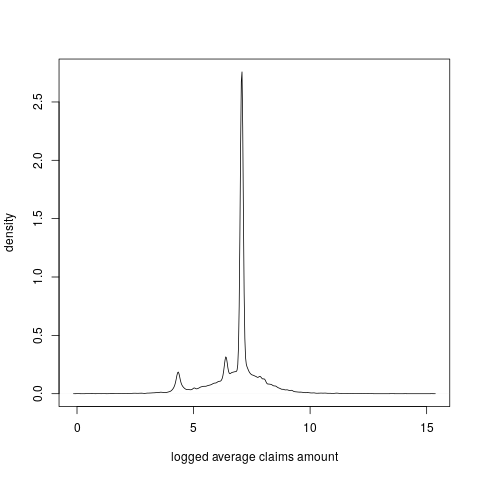
\includegraphics[width=0.45\linewidth]{../plots/sev/hist.png}
		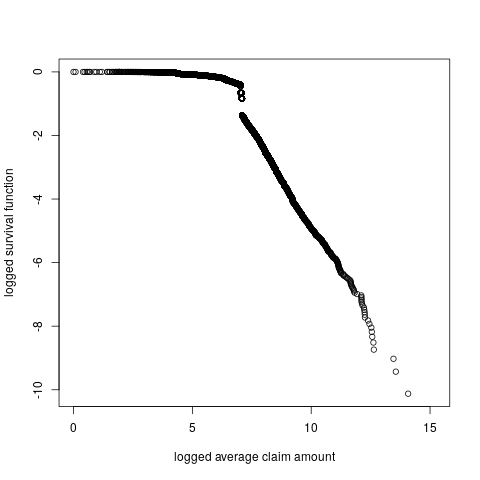
\includegraphics[width=0.45\linewidth]{../plots/sev/log-log.png}
		\caption{Histogram and logged survival function of logged average claims.}\label{tail}
	\end{figure}
An intuitive choice of component distributions is that 
three peaks are modelled by three gamma distributions, respectively, the resting non-tail part by a forth gamma distribution, and the tail part by a Pareto distribution.
Therefore, the probability density function (of the null model) is given by
\begin{equation}\label{sev-0}
	f(Y|\bx;p,\mu,\phi,\alpha)=\sum_{k=1}^4p_kf_{G}(Y;\mu_k,\phi_k)+p_5f_{P}(Y;\alpha,M)
\end{equation}

	where $\mu,\phi$ are mean and dispersion parameter, and $\alpha, M$ are tail index and threshold. The threshold is pre-determined as $8158.13$ according to Hill plot.
	
	Figure \ref{tail} indicates a way to initialize the hidden variable:
	\begin{equation}
		\begin{aligned}
			\hat{z}^{[0]}_i&=(\hat{z}^{[0]}_{i,1},\hat{z}^{[0]}_{i,2},\hat{z}^{[0]}_{i,3},\hat{z}^{[0]}_{i,4},\hat{z}^{[0]}_{i,5})^\top\\
			&=(\mathbbm{1}_{(0,500]}y_i,\mathbbm{1}_{(500, 1000]}y_i,\mathbbm{1}_{(1000,1200]}y_i,\mathbbm{1}_{(1200,8158.13]}y_i,\mathbbm{1}_{(8158.13,\infty)}y_i)^\top
		\end{aligned}
	\end{equation}
	Other parameters can be initialized as the MLE based on the full likelihood function.
We first fit a null model \eqref{sev-0} to the data via the EM algorithm. 
The trace of learning loss is shown in Figure \ref{null_sev}.
	\begin{figure}[h!]
		\centering
		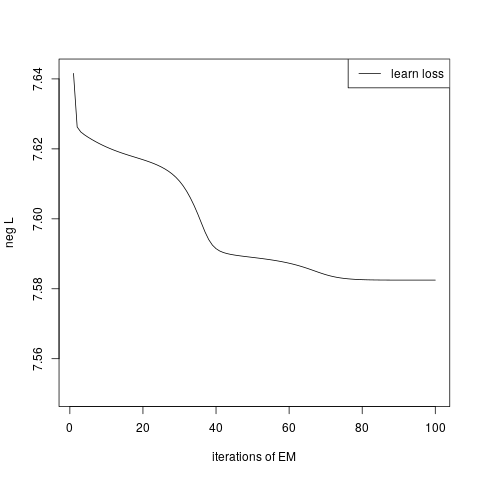
\includegraphics[width=0.5\linewidth]{../plots/sev/null_trace}
		\caption{Learning loss of mixture of distributions.}\label{null_sev}
	\end{figure}
The estimated parameters are listed in Table \ref{null-gamma}. We observe that three peaks are captured by the first three component gamma distributions.
	\begin{table}[h!]
		\centering
		\caption{MLE of four component gamma distributions. Tail index is estimated as $\hat{\alpha}=1.0773$.}\label{null-gamma}
		\begin{tabular}{crrrr}
			\hline
			component $k$ & \multicolumn{1}{c}{$\mu_k$} & \multicolumn{1}{c}{shape $(1/\phi_k)$} & \multicolumn{1}{c}{scale} & \multicolumn{1}{c}{rate} \\ \hline
			1         & 76.8727                & 105.556                   & 0.7283                    & 1.3731                   \\
			2         & 592.5909               & 653.539                   & 0.9067                    & 1.1029                   \\
			3         & 1171.3811              & 999.9999                  & 1.1714                    & 0.8537                   \\
			4         & 1534.5143              & 1.0377                    & 1478.7768                 & 7e-04                    \\ \hline
		\end{tabular}
	\end{table}
	Those large shape parameters (small dispersion) implies the  difficulties with {gamma mean modeling}. The test loss is calculated as 7.5815.

Next we model the mixing probabilities by boosting algorithm:
\begin{equation}\label{sev-bst-p}
f(Y|\bx;p,\mu,\phi,\alpha)=\sum_{k=1}^4p_k(\bx)f_{G}(Y;\mu_k,\phi_k)+p_5(\bx)f_{P}(Y;\alpha,M).
\end{equation}
We draw the boxplot of the mixing probabilities in Figure \ref{bx-bst-p}, which implies that the mixing probabilities of third and forth components $p_3$ and $p_4$ are more related with the covariates.
The test loss is calculated as 7.5588 smaller than the null model.
	\begin{figure}[htp!]
		\centering
		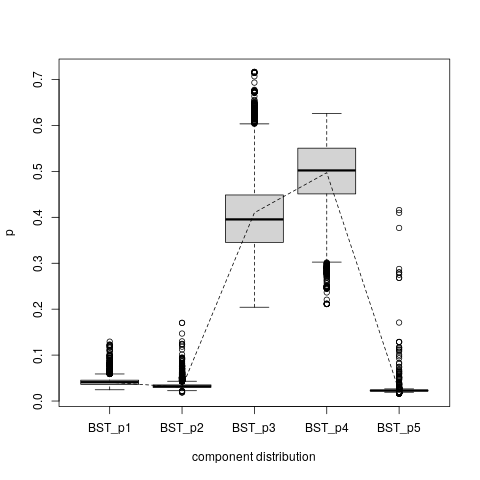
\includegraphics[width=0.35\linewidth]{../plots/sev/bst_p}
		\caption{Boxplot of estimated mixing probabilities.}\label{bx-bst-p}
	\end{figure}


The small shape parameter of the forth component as shown in Table \ref{null-gamma} indicates a possible improvement by boosting the forth component  mean.
Therefore, we fit the following model:
	$$
	\begin{aligned}
		f(Y|\bx;p,\mu,\phi,\alpha)=&\sum_{k=1}^3p_k(\bx)f_{G}(Y;\mu_k,\phi_k)+ \\
		&p_4(\bx)f_{G}(Y|\bx;\mu_4(\bx),\phi_4)+ p_5(\bx)f_{P}(Y;\alpha,M).
	\end{aligned}
	$$
	Test loss is calculated as 7.5573 smaller than that of model \eqref{sev-bst-p}. 


\section{Conclusions}\label{sec:conclusions}
Insurance loss data sometimes cannot be sufficiently modelled by a single distribution.
Those data is usually modelled by mixture of models.
The traditional estimation method for mixture of models is the EM algorithm.
However, thee EM algorithm is not quite useful when the component model is supposed to be non-parametric.
In this paper, we propose an Expectation-Boosting (EB) algorithm for mixture of models, where both the mixing probabilities and the component models are supposed to be modelled non-parametrically. 
The proposed algorithm replaces the maximization step of the EM algorithm by a generic functional gradient descent algorithm.
There are several advantages of EB algorithm over the EM algorithm. 
First, boosting algorithm is a flexible non-parametric regression facilitating both {non-linear effects and interaction}.  
There is no need for specifying the form of component regression functions and performing covariate transformation, which is difficult in the mixture of models.
Second, boosting algorithm is {overfitting-sensitive}, we can perform {variable selection} simultaneously during the EB algorithm.
In this paper, we do not discuss the model interpretation, which is quite similar to those in normal boosting algorithm, such as variable importance, ice curve, etc. 
We discuss number of components selection ad hoc rather than systematically.
One may refer to ?? for more details.


\bibliography{boosting}
\bibliographystyle{boosting}

\end{document}
